\documentclass{article}
\usepackage{graphicx}
\usepackage{listings}
\usepackage{siunitx}
\usepackage{placeins} %chatGPT suggestion to prevent figures getting rendered weirdly

\setlength{\topmargin}{-2cm} 
\setlength{\textheight}{650pt}
\begin{document}

\section*{Implementation}
Implementation went very smoothly and I used ChatGPT in a similar way as the last homework
to help understand some matplotlib and numpy documentation. I ran into no issues until plotting myself
but that was quickly resolved. I spent the majority of the time on this project figuring out how to make
my phase space plot more clear since it was nothing but a blob of color with default values
to do this I had ChatGPT explain the color map argument for matplotlib and after looking at a few cmap options
I decided on 'tab10' because it had 10 unique hues which is the same as the \# of initial conditions we have in our 
ensemble

\section*{Questions}
\subsection*{1. Include all of the plots that you generated as figures in your report.}
    \begin{figure}[htbp]
        \centering
        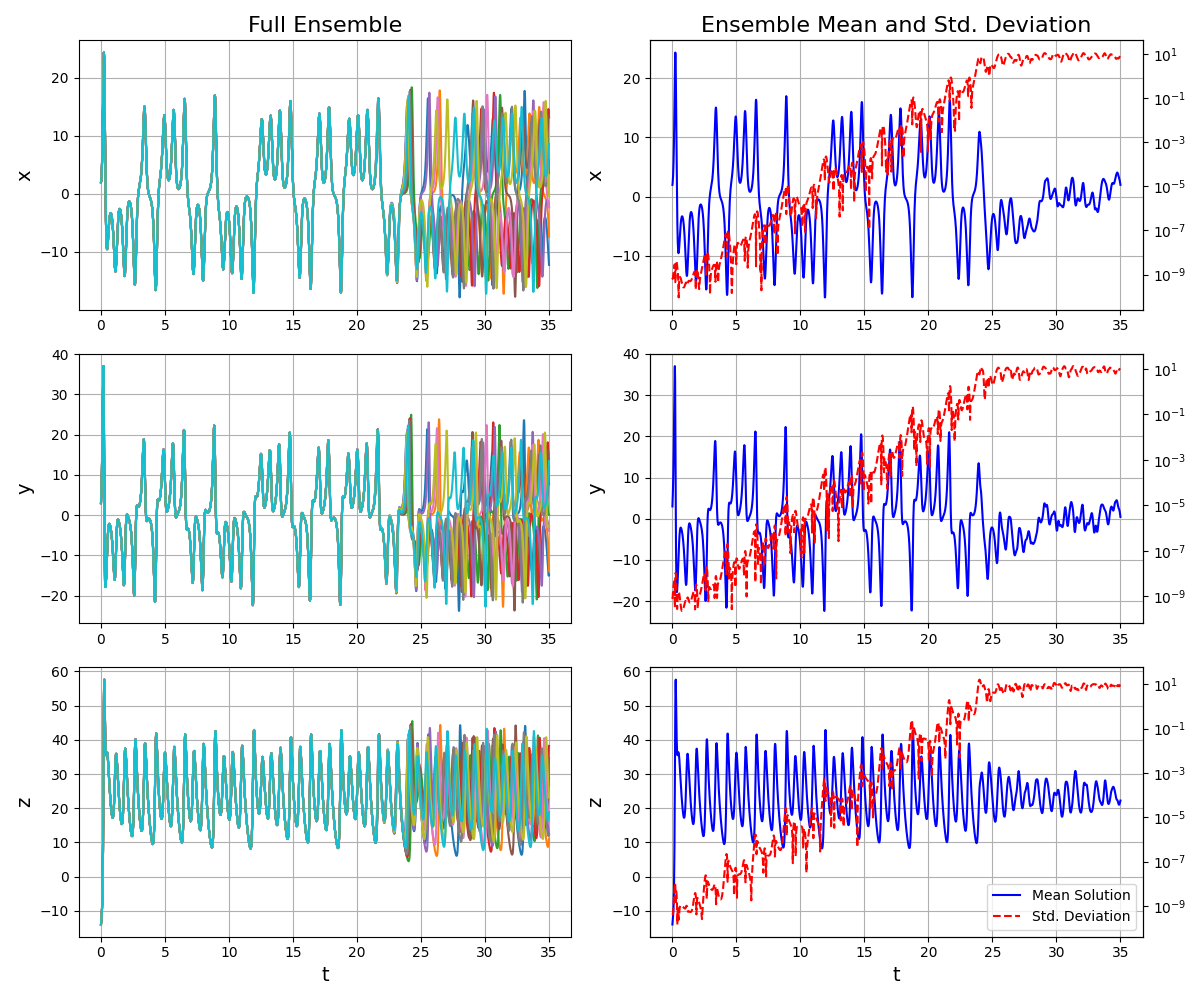
\includegraphics[width=0.8\textwidth]{../solutions.png}
        \caption{Solution of the full ensemble and the mean of the ensemble projected onto the x, y , and z planes}
        \label{fig: solutions.png}
    \end{figure}
    
    \begin{figure}[htbp]
        \centering
        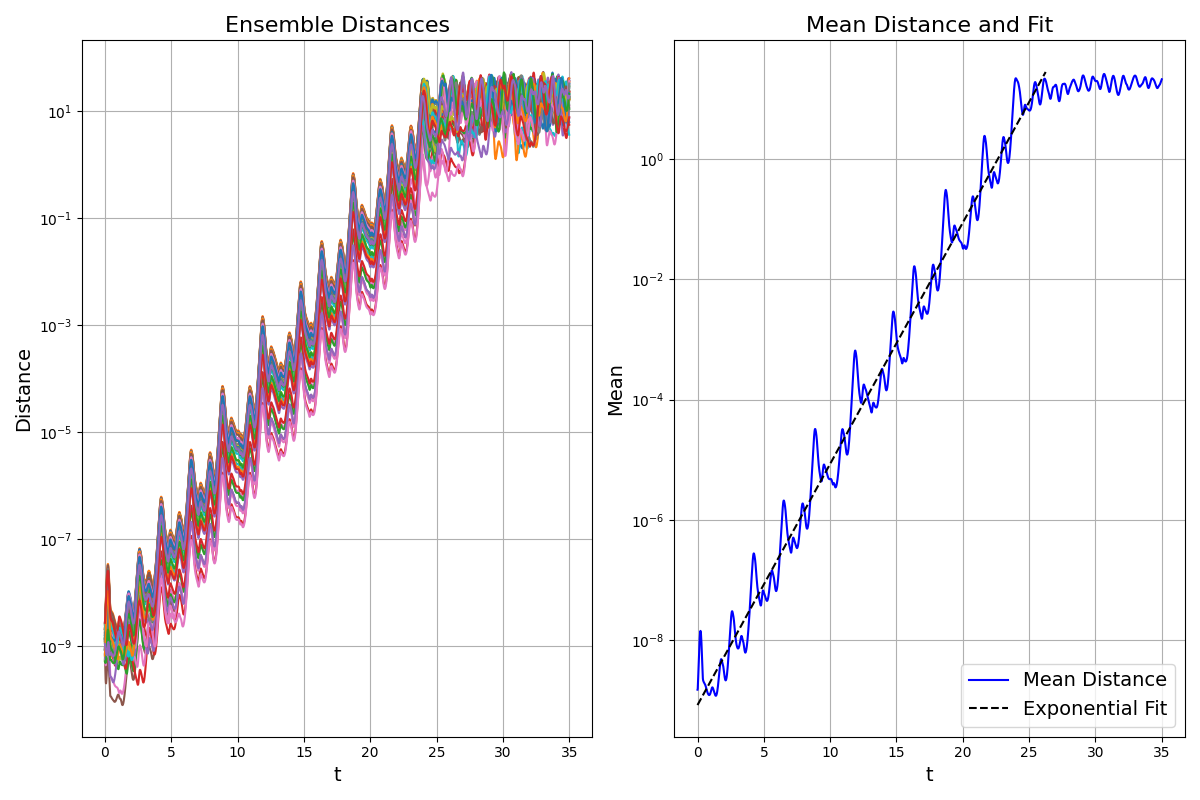
\includegraphics[width=0.8\textwidth]{../distances.png}
        \caption{Distance and Mean distance over time}
        \label{fig: distances.png}
    \end{figure}

    \begin{figure}[htbp]
        \centering
        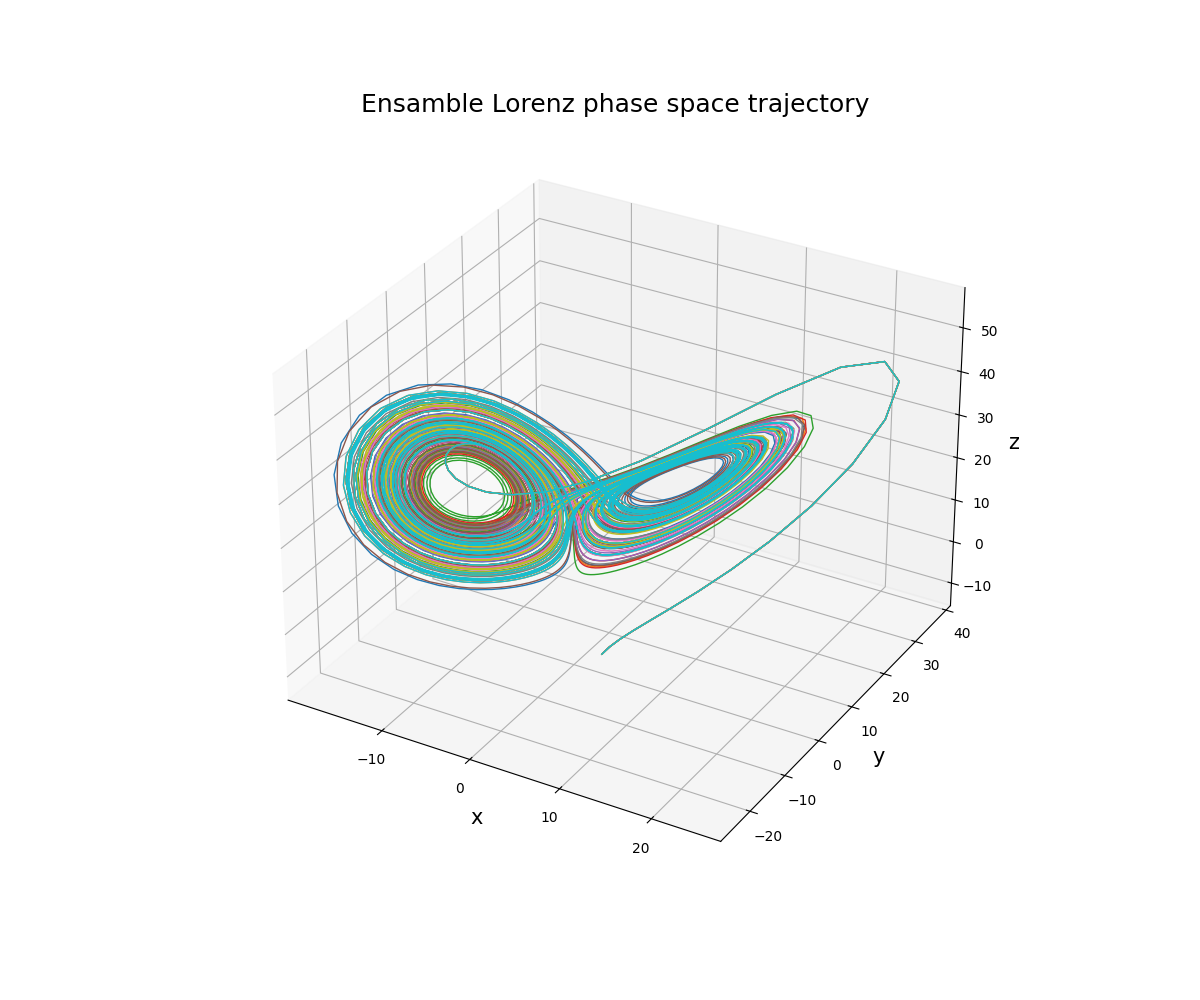
\includegraphics[width=0.8\textwidth]{../phaseSpace.png}
        \caption{3d phase space plot}
        \label{fig: phaseSpace.png}
    \end{figure}

    \FloatBarrier

\subsection*{2. Discuss how we managed multiple solutions to the same IVP.}
we defined a set of initial conditions and then iteratively solved the IVP at each initial condition adding that solution to a list of solutions
the solutions are unique despite how close together all the initial conditions are cause of the property of the lorenz equations that similar initial
conditions rapidly diverge, the solutions are stored in a list of numpy arrays and where the each numpy array is a 3x(number of time steps) matrix
they are implicitly aligned with time because we plot it over a predefined array of time where both have the same amount of time steps

\subsection*{3. Discuss how the ensembleStats function works}
\lstinline|ensembleStats| takes the list of solutions and finds the average solution as well as the standard deviation from that average
this lets us see that the standard deviation starts very low and grows over time until a point after which it stays relatively constant.
this observation can also be seen mirrored on all 3 axis as well as in the distances plot. The \lstinline|ensembleStats| function makes use of 
mumpy array arithmetic so as long as the argument being passed is a list of numpy arrays then it should work to find the mean and the standard deviation
which is why it can be used in both \lstinline|plotDistances| and \lstinline|plotEnsemble|

\subsection*{4. Explain how you calculated the distance between two solutions. Did using NumPy arrays make this easy?}
We take the vector difference of all the solutions with all the other solutions (avoiding double counting and self comparison) which gives us a list of NumPy arrays
which contains the difference in the z, y, and z between every time point of every solution. We can then use \lstinline|np.linalg.norm| to get a list of numpy Arrays containing the
distance between points at every time and every solution

\subsection*{5. Report the Lyapunov exponent that your code predicts. How close is it to the known digits from analysis?}
my predicted Lyapunov exponent is: 0.918963. this result is within 0.02 of the known digits, the accuracy of our predicted value can be 
marginally improved by running with more initial conditions at the cost of runtime

\subsection*{6. Finally, discuss your additional plot.}
I chose my additional plot to be the phase space plot which is plotting similar information as the solutions plot but it 
plots it in 3d without an explicit time axis. with the help of GPT I color coded the plot to make each solution more clear. 
If you examine the plot you notice that all the solutions appear to be initially stacked on top of each other 
as you can only see one color, but as the solutions start to spiral inwards they diverge and you can see the unique colors

\end{document}
